\documentclass[11pt,aspectratio=169,handout]{beamer}

\usetheme{Singapore}
\usecolortheme{orchid}

\usepackage[utf8]{inputenc}
\usepackage[russian]{babel}
\usepackage{amsmath}
\usepackage{amsfonts}
\usepackage{amssymb}
\usepackage{graphicx}
\usepackage{bibentry}
\usepackage{wasysym}
\usepackage[most]{tcolorbox}
\usepackage[normalem]{ulem}

\usepackage{hyperref}

\definecolor{info}{RGB}{62, 180, 137}
\definecolor{warn}{RGB}{128, 0, 0}

\author{Николай Анохин}
\title{Нейросетевые рекомендеры I: \\ отбор кандидатов}

\logo{
\includegraphics[width=.05\textwidth]{images/ok_logo.png}}

\AtBeginSection[]{
  \begin{frame}
  \vfill
  \centering
  \begin{beamercolorbox}[sep=8pt,center,shadow=true,rounded=true]{title}
    \usebeamerfont{title}\insertsectionhead\par
  \end{beamercolorbox}
  \vfill
  \end{frame}
}

\begin{document}

{
\setbeamertemplate{headline}{}

\begin{frame}
\titlepage
\end{frame}

%\begin{frame}
%\tableofcontents
%\end{frame}

}

\begin{frame}{Контекст}

\begin{center}
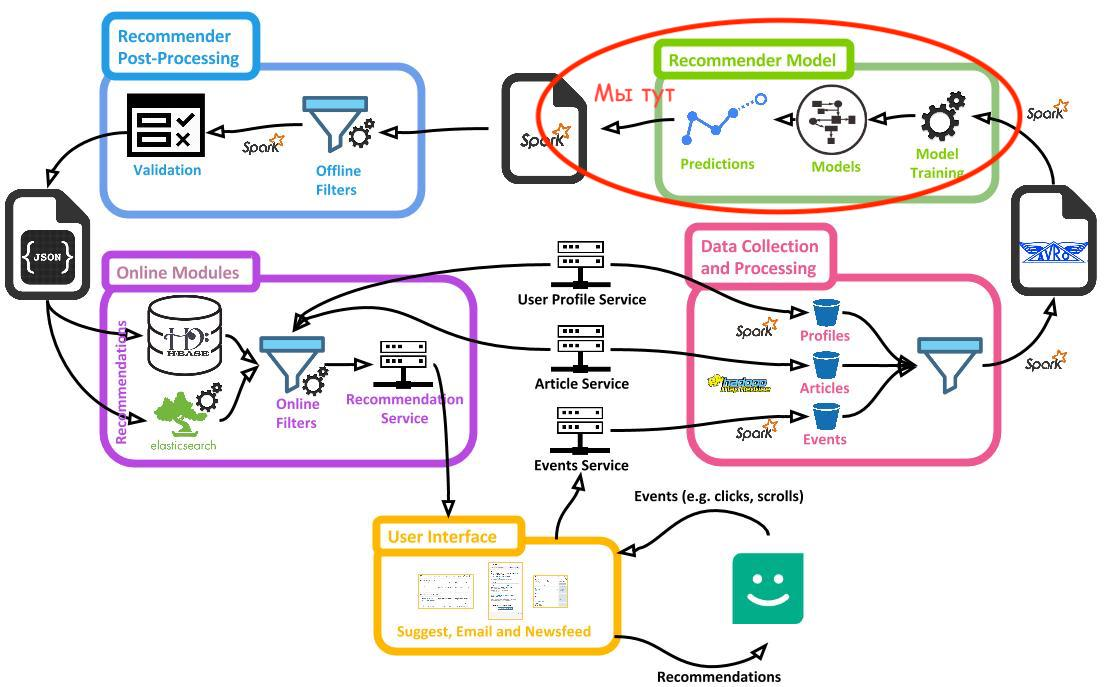
\includegraphics[scale=0.23]{images/mendeley.jpeg}
\end{center}

\end{frame}

\section{От классики к нейросетям}

\begin{frame}{От классики к нейросетям}

\begin{columns}
\begin{column}{0.4\textwidth} 
\begin{center}
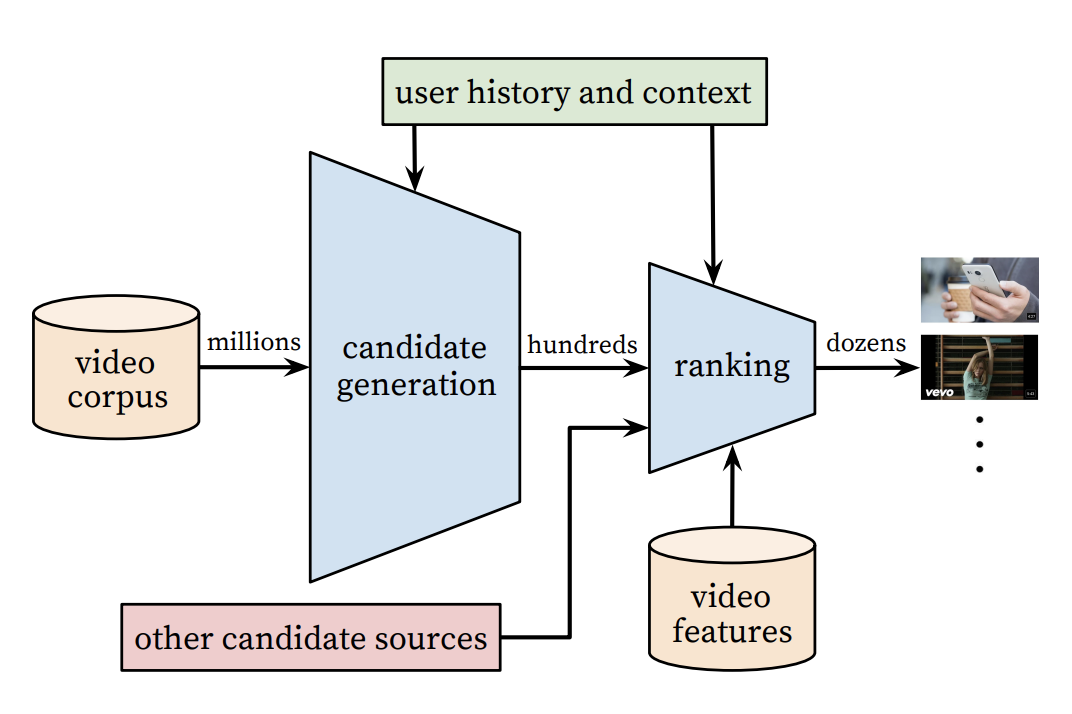
\includegraphics[scale=0.3]{images/youtube-arch.png}
\end{center}
\end{column}
\begin{column}{0.5\textwidth}

\begin{small}
\begin{tabular}{l c c}
 & Классика & Нейросетевые \\
\hline
Отбор кандидатов & MF & NN \\
Ранжирование & GBM & NN
\end{tabular}

\begin{center}
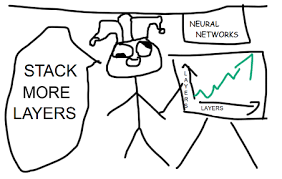
\includegraphics[scale=0.5]{images/layers.png}
\end{center}

\end{small}

\end{column}
\end{columns}

\end{frame}

\begin{frame}

\begin{columns}
\begin{column}{0.47\textwidth}
\begin{center}
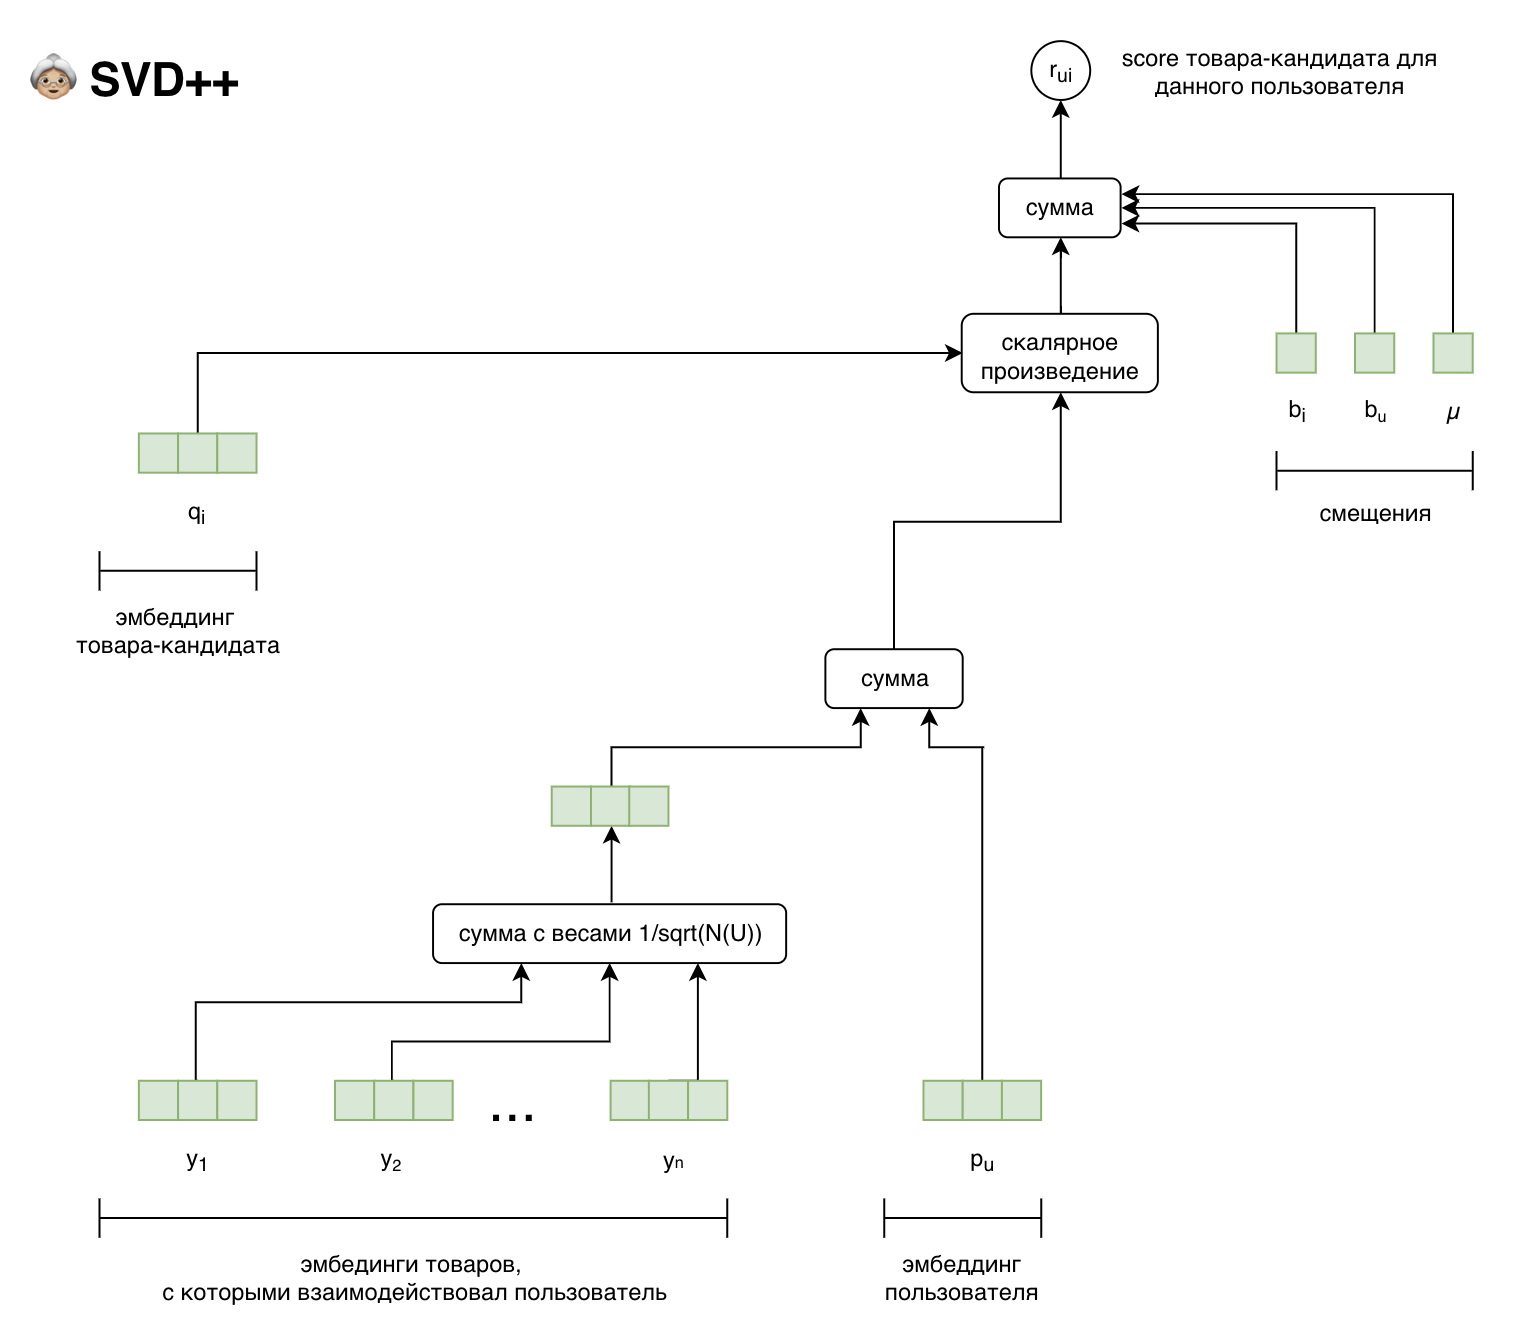
\includegraphics[scale=0.25]{images/svdpp.png}
\end{center}
\end{column}
\begin{column}{0.47\textwidth}
\begin{small}
\[
\hat r_{ui} = \mu + b_u + b_i + q_i^T \left( p_u + \frac{1}{\sqrt{|N(u)|}} \sum_j y_j \right)
\]
\end{small}
\end{column}
\end{columns}

\end{frame}

\begin{frame}

\begin{columns}
\begin{column}{0.47\textwidth} 
\begin{center}
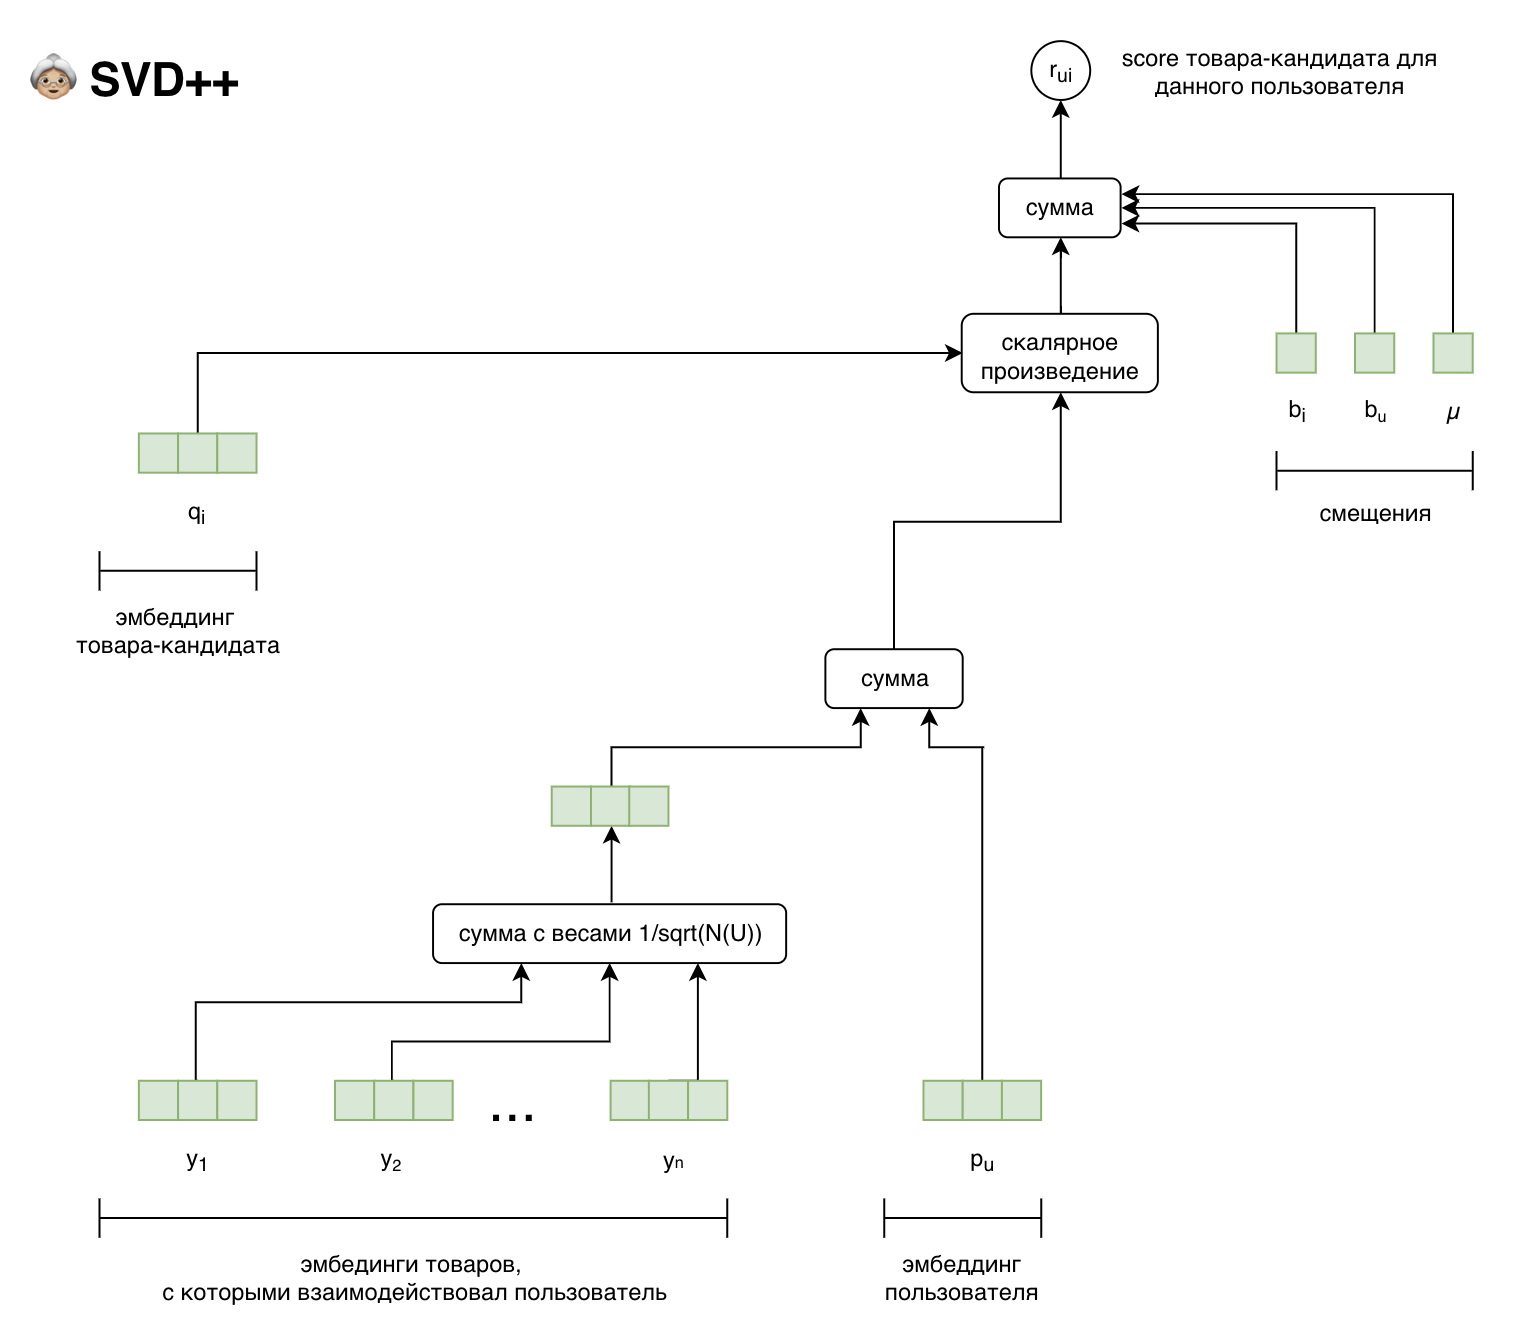
\includegraphics[scale=0.25]{images/svdpp.png}
\end{center}
\end{column}
\begin{column}{0.47\textwidth}
\begin{center}
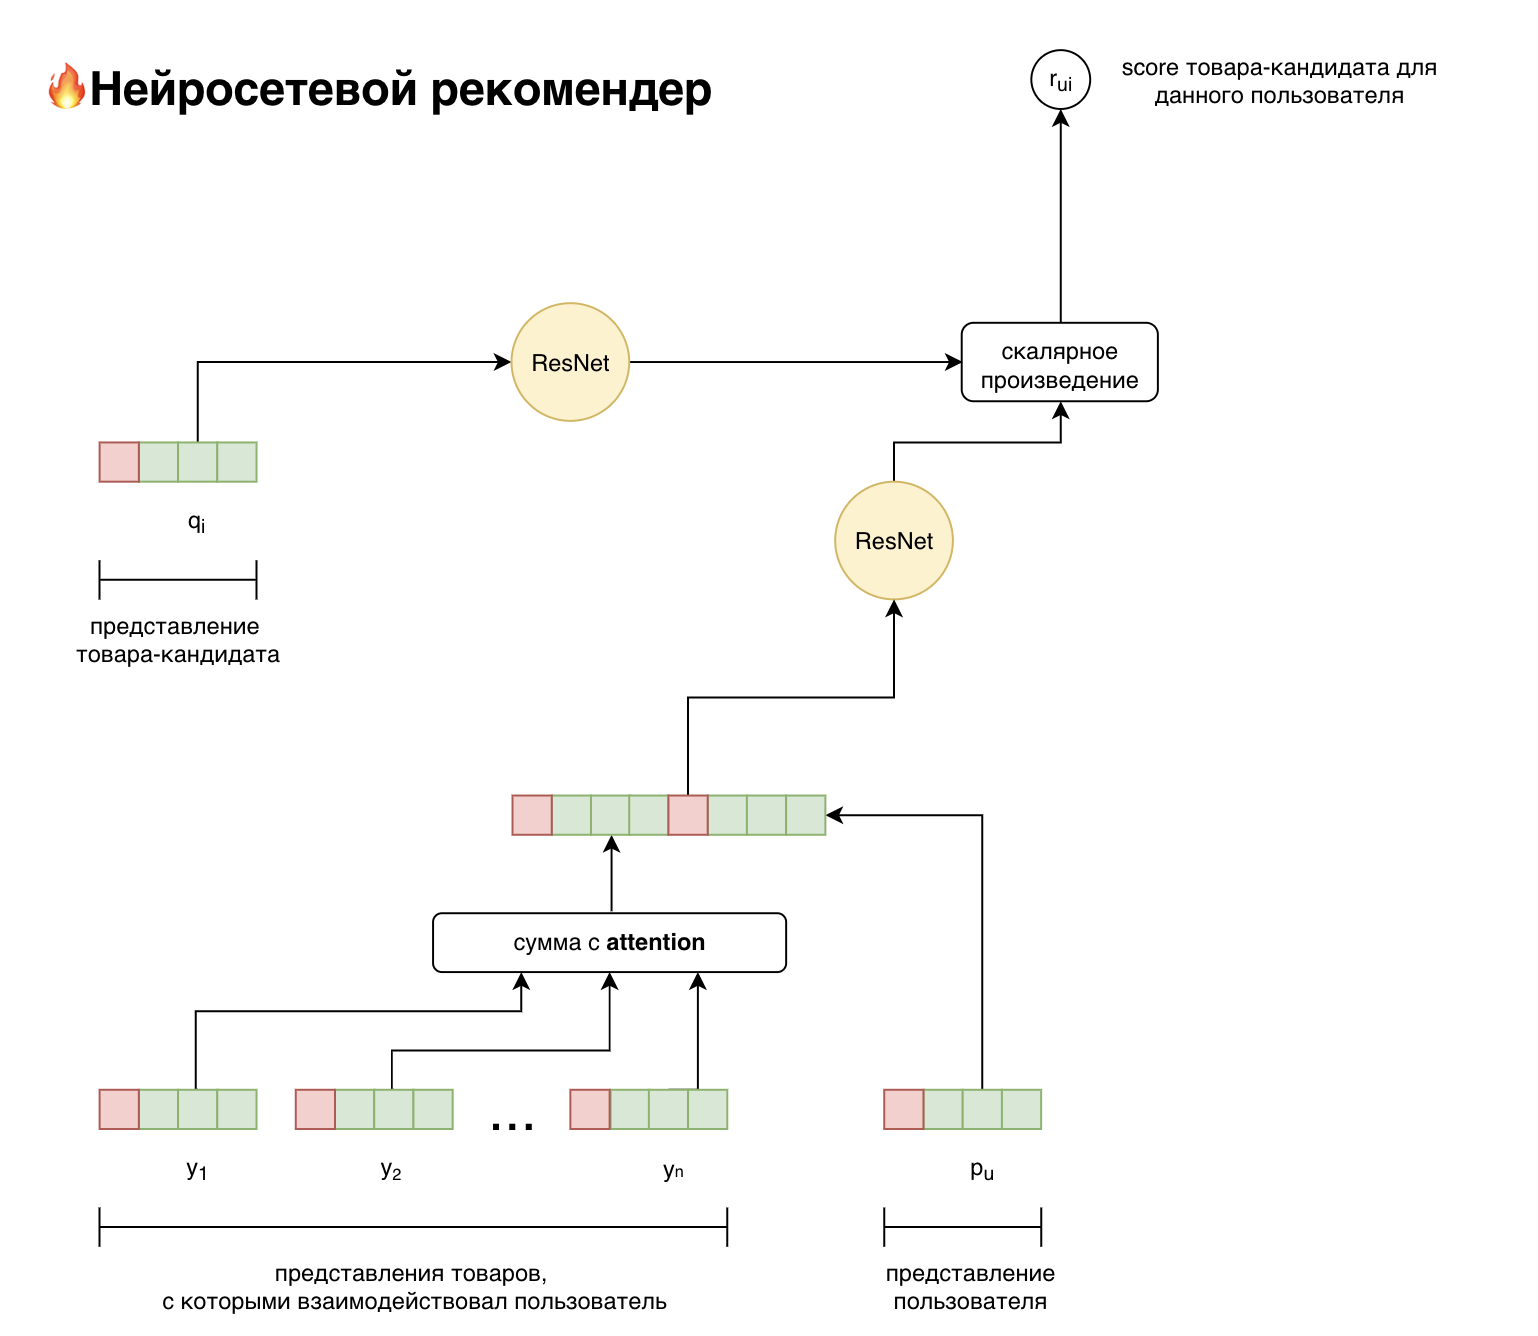
\includegraphics[scale=0.25]{images/nn.png}
\end{center}
\end{column}
\end{columns}

\end{frame}

\section{Истории успеха: отбор кандидатов}

\begin{frame}{Истории успеха\footnote{Но это не точно}: отбор кандидатов}

ML = модель + лосс + алгоритм оптимизации + данные

\vfill

\begin{tcolorbox}[colback=info!5,colframe=info!80,title=Как оставить след в науке]
\pause
\begin{itemize}[<+->]
\item Заменить скалярное произведение чем-нибудь покруче
\item Заменить эмбединги чем-нибудь покруче
\item Изобрести или прикрутить хитрый лосс
\item Изобрести новый метод сэмплирования данных
\end{itemize}
\end{tcolorbox}

\end{frame}

\begin{frame}{Neural Collaborative Filtering \cite{NCF}}

\begin{columns}
\begin{column}{0.45\textwidth} 
\begin{center}
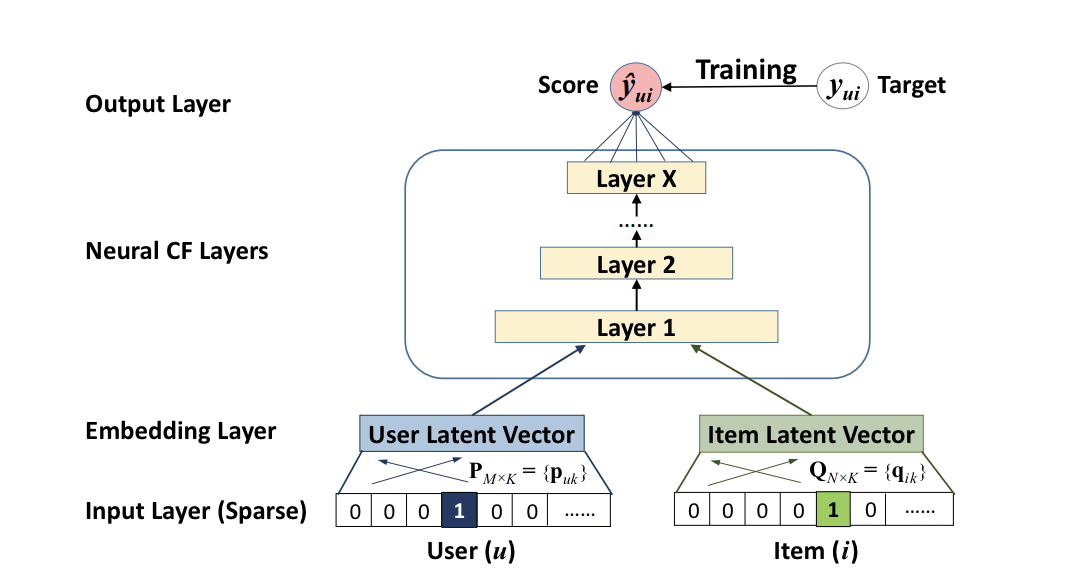
\includegraphics[scale=0.35]{images/ncf.png}
\end{center}
\end{column}
\begin{column}{0.45\textwidth}
\begin{center}
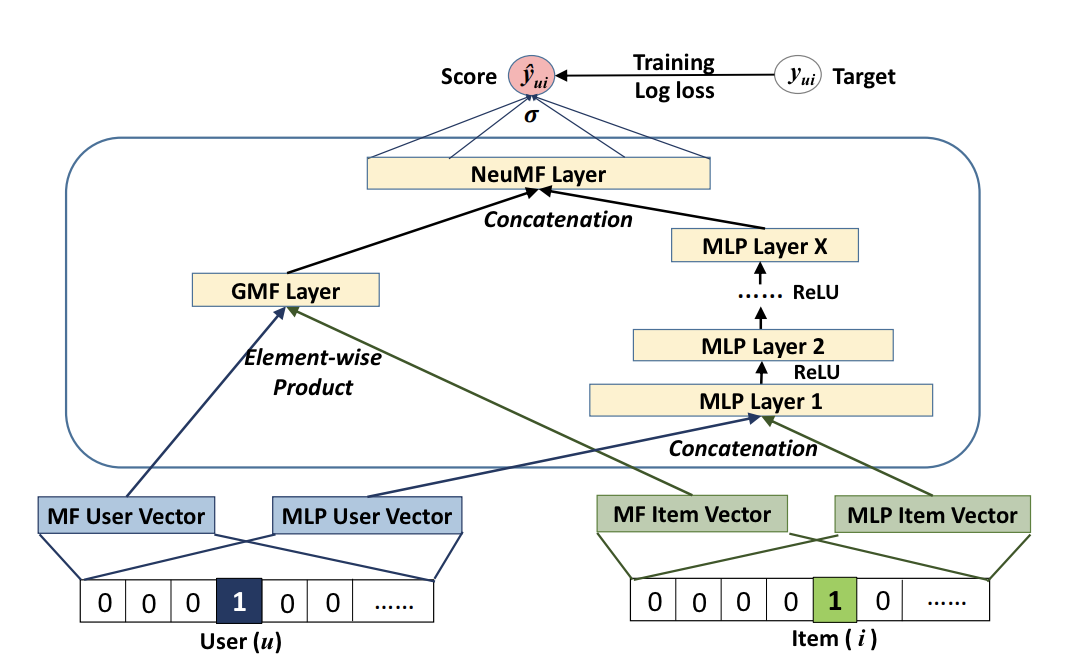
\includegraphics[scale=0.35]{images/nfm.png}
\end{center}
\end{column}
\end{columns}

\begin{tabular}{l l}
Интересность & $\star\star\star$ \\
Полезность & $\star\star\star$
\end{tabular}

\end{frame}

\begin{frame}{Learning Deep Structured Semantic Models for Web Search using Clickthrough Data \cite{DSSM}}

\begin{center}
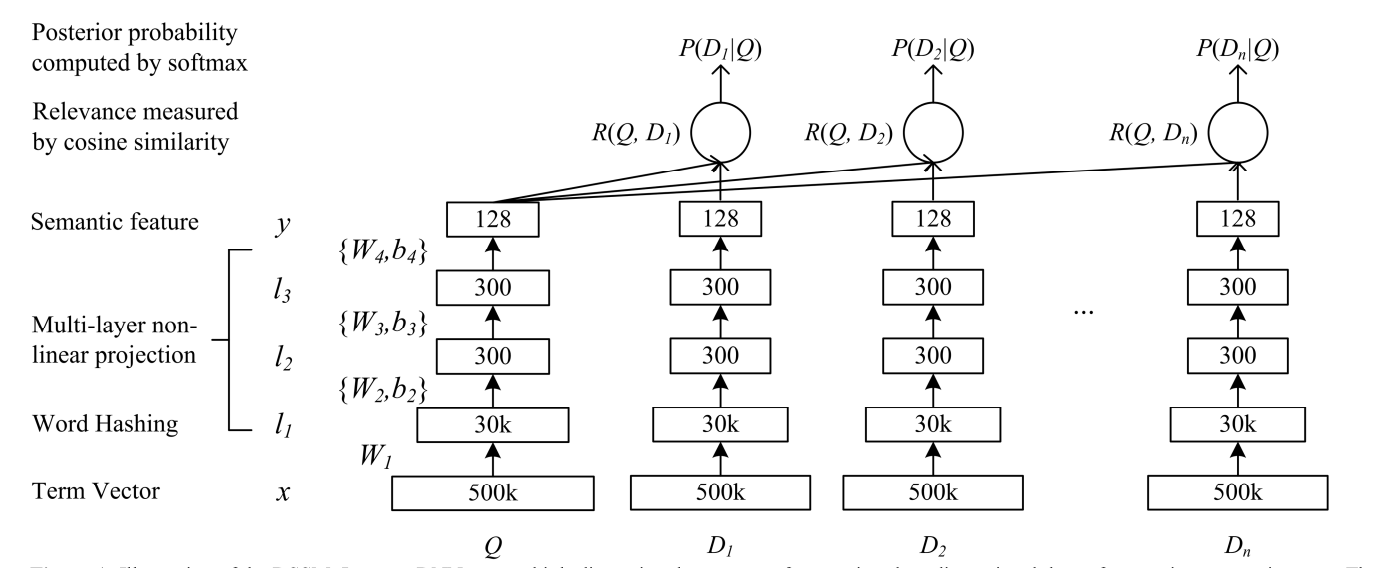
\includegraphics[scale=0.35]{images/dssm.png}
\end{center}

\begin{tabular}{l l}
Интересность & $\star\star\star$ \\
Полезность & $\star\star\star\star$
\end{tabular}

\end{frame}

\begin{frame}{Deep Neural Networks for YouTube Recommendations \cite{YTBE}}

\begin{center}
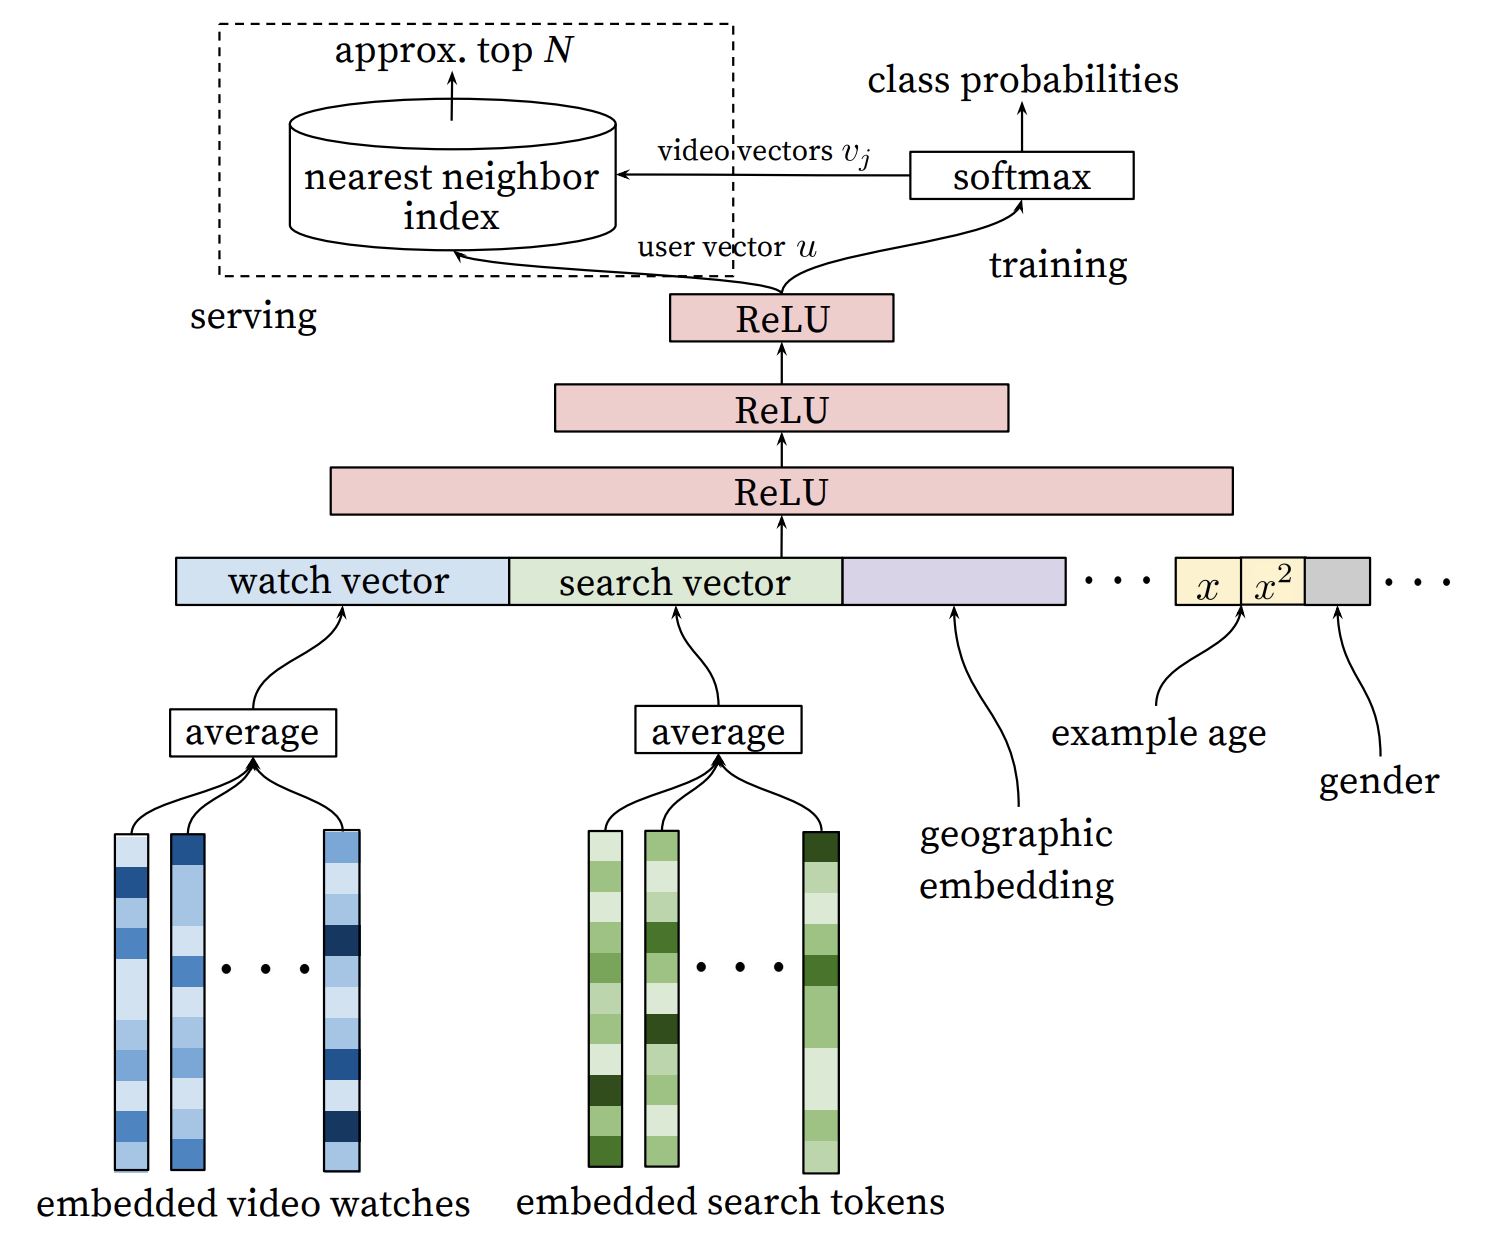
\includegraphics[scale=0.25]{images/youtube-candidate.png}
\end{center}

\begin{tabular}{l l}
Интересность & $\star\star\star\star\star$ \\
Полезность & $\star\star\star\star\star$
\end{tabular}

\end{frame}

\begin{frame}{BERT4Rec: Sequential Recommendation with Bidirectional Encoder Representations from Transformer \cite{BERT4Rec}}

\begin{center}
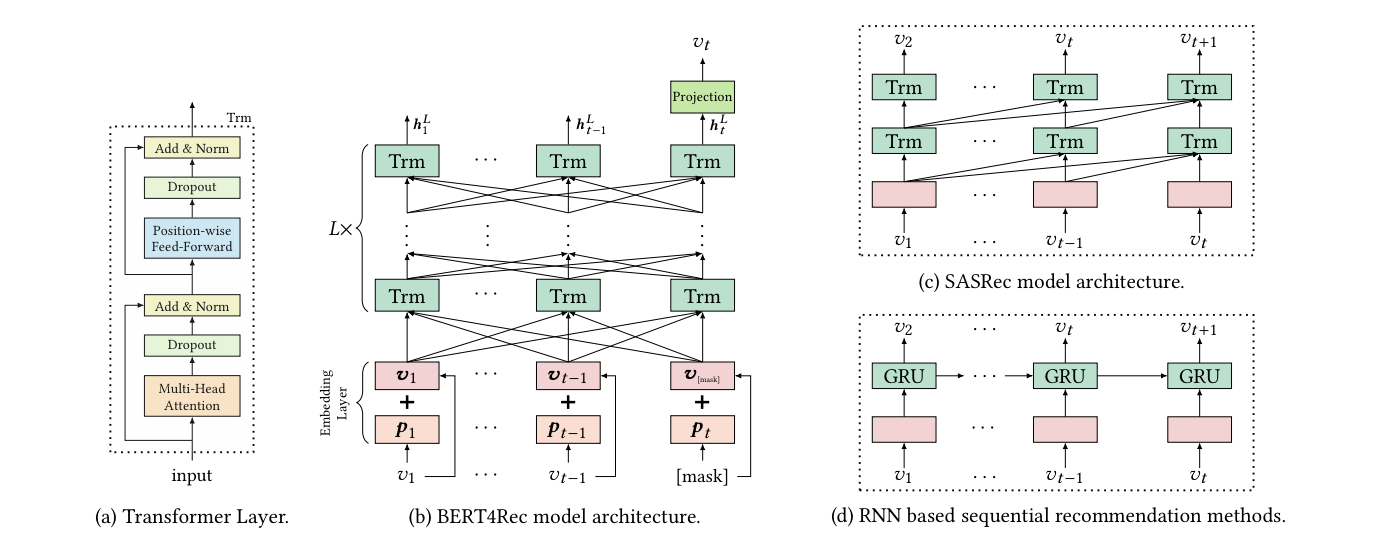
\includegraphics[scale=0.4]{images/bert4rec.png}
\end{center}

\begin{tabular}{l l}
Интересность & $\star\star$ \\
Полезность & $\star$
\end{tabular}

\end{frame}

\begin{frame}{BERT4Rec: эксперименты}

\begin{center}
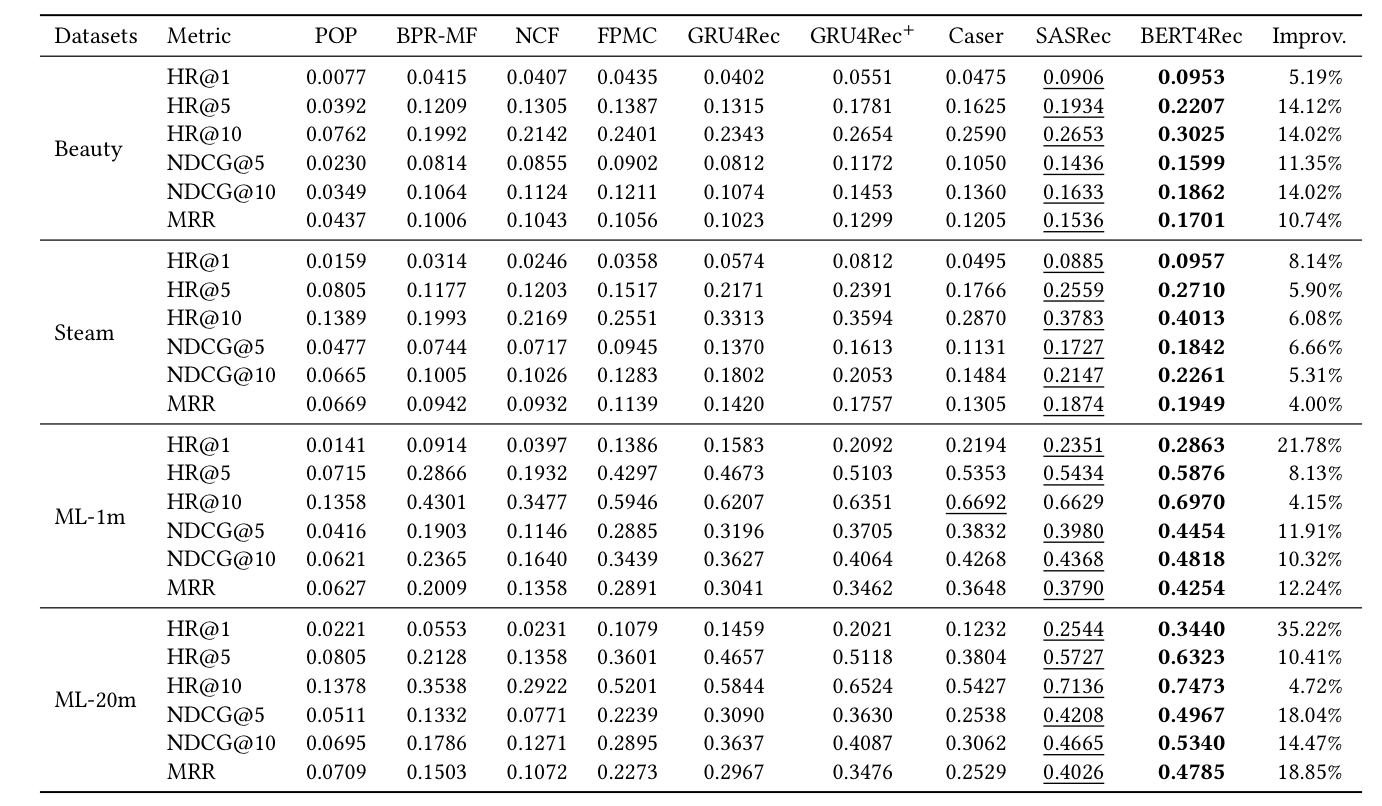
\includegraphics[scale=0.45]{images/bert4rec-table.png}
\end{center}

\end{frame}

\begin{frame}{Deep Feedback Network for Recommendation \cite{DFN}}

\begin{center}
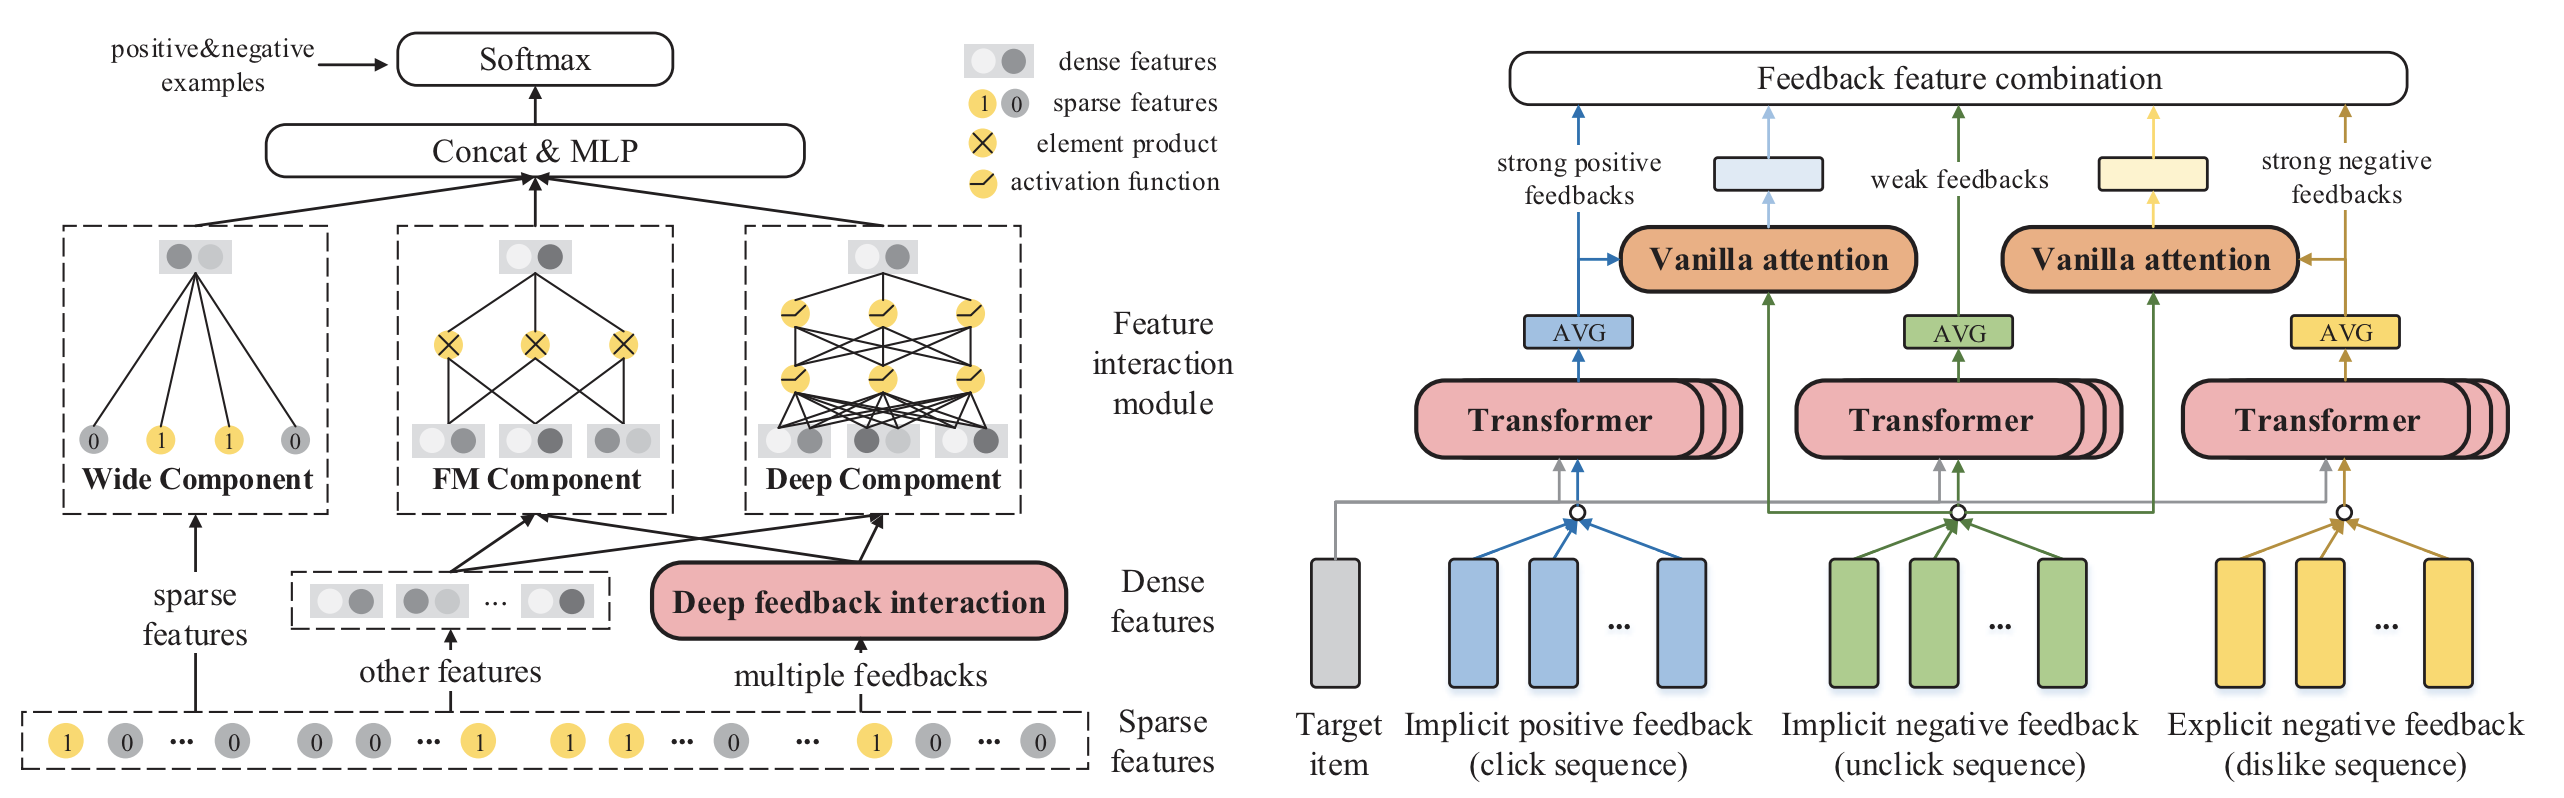
\includegraphics[scale=0.3]{images/dfn.png}
\end{center}

\begin{tabular}{l l}
Интересность & $\star\star\star$ \\
Полезность & $\star$
\end{tabular}

\end{frame}

\begin{frame}{Self-supervised Learning for Large-scale Item Recommendations \cite{SSL}}

\begin{columns}

\begin{column}{0.45\textwidth} 
\begin{center}
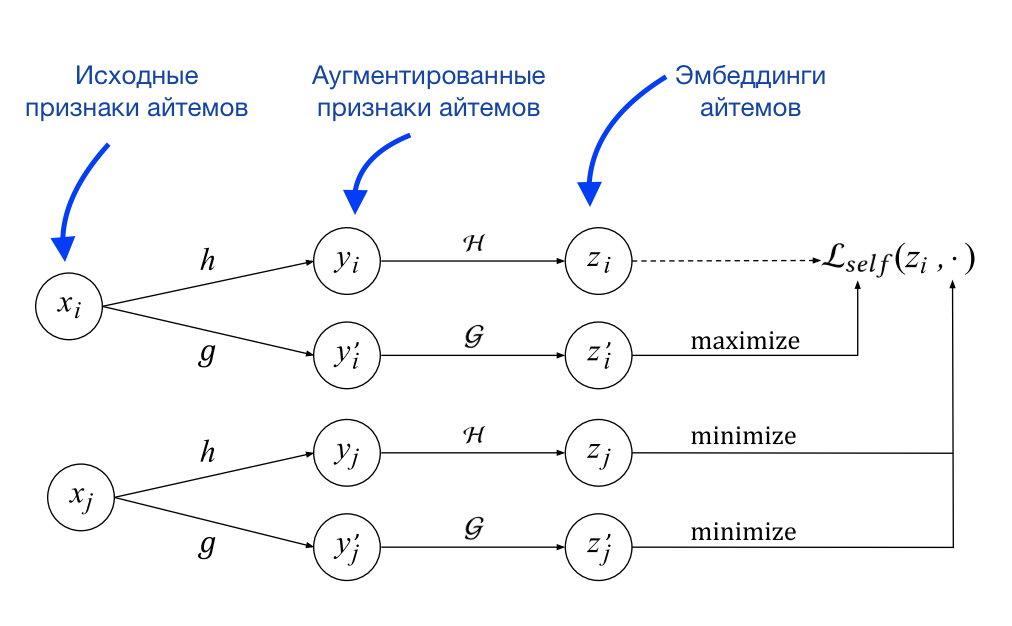
\includegraphics[scale=0.35]{images/ssl.png}
\end{center}
\end{column}

\begin{column}{0.45\textwidth}

\begin{small}
{\bf Аугментации}
\begin{itemize}
\item {\it Masking.} С некоторой вероятность маскируем (скореллированные) признаки айтемов.
\item {\it Dropout.} С некоторой вероятностью зануляем категории в мульти-категориальных признаках.
\end{itemize}
\end{small}

\end{column}
\end{columns}

\vfill

\begin{tabular}{l l}
Интересность & $\star\star\star\star$ \\
Полезность & $\star\star\star$
\end{tabular}

\end{frame}

\section{Что работает на практике}

\begin{frame}{Сбор данных для модели \cite{METH}}

\begin{itemize}
\item {\bf Positives} \\ клики, покупки
\item {\bf Simple negatives} \\ случайные айтемы
\item {\bf Hard negatives} \\ айтемы, прошедшие отбор кандидатов, но не прошедшие ранкер
\end{itemize}

\end{frame}

\begin{frame}{Архитектуры \cite{METH}}

\begin{itemize}
\item Two-tower model
\item DCNv2 (в следующий раз)
\item Архитектуры с отдельными выходами под каждый таргет (клик, лайк и т.д.)
\item Sampling-bias correction \& Self-supervised learning
\end{itemize}

\end{frame}

\begin{frame}{Item-to-Item (i2i)\footnote{i2i в Дзене \url{https://t.me/mlvok/39}}}

Шаг 1: $user \rightarrow item$ -- получаем айтемы $I_U$, которыми интересовался пользователь \\
Шаг 2: $item \rightarrow item$ -- получаем айтемы, похожие на $I_U$

\vfill

Индексы для приближенного поиска ближайших соседей\footnote{\url{https://ann-benchmarks.com/}}
\begin{center}
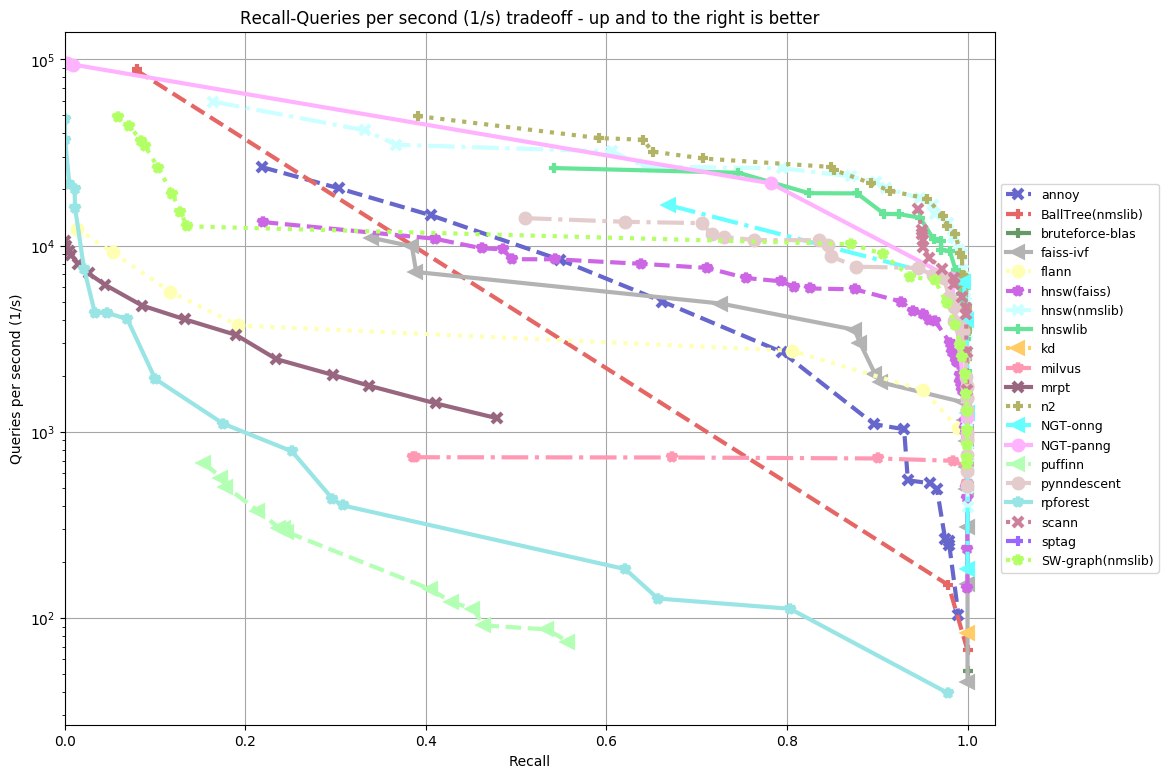
\includegraphics[scale=0.2]{images/ann.png}
\end{center}

\end{frame}

\section{Итоги}

\begin{frame}{Итоги}

\begin{tcolorbox}[colback=info!5,colframe=info!80,title=]
Нейросетевые модели могут заменить любой компонент рекомендательной системы: отборщик кандидатов, ранкер, item2item.
\end{tcolorbox}

\vfill

\begin{tcolorbox}[colback=info!5,colframe=info!80,title=]
Посмотрели на популярные идеи для нейросетевых отборщиках кандидатов и обсудили, что работет на практике.
\end{tcolorbox}

\end{frame}

\begin{frame}
\begin{center}

\includegraphics[scale=1.0]{images/bye.jpeg}
\end{center}
\end{frame}

\begin{frame}{Подпишись скорее}

\begin{columns}
\begin{column}{0.45\textwidth}
   \begin{center}
                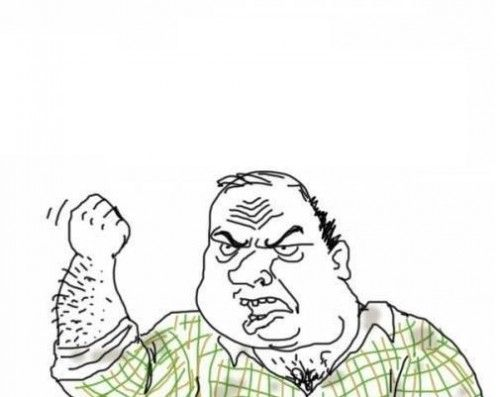
\includegraphics[scale=0.3]{images/ble.jpeg}
   \end{center}
\end{column}
\begin{column}{0.45\textwidth}
   \begin{center}
                \url{https://t.me/mlvok}

                
\includegraphics[scale=0.5]{images/tgqr.png}
   \end{center}
\end{column}
\end{columns}

\end{frame}

\begin{frame}[allowframebreaks]{Литература}

\bibliographystyle{amsalpha}
\bibliography{references.bib}

\end{frame}

\end{document}
